% % fancy table template:
% \begin{tabular}{ |p{3cm}||p{3cm}|p{3cm}|p{3cm}|  }
%  \hline
%  \multicolumn{4}{|c|}{Country List} \\
%  \hline
%  Country Name or Area Name& ISO ALPHA 2 Code &ISO ALPHA 3 Code&ISO numeric Code\\
%  \hline
%  Afghanistan   & AF    &AFG&   004\\
%  Aland Islands&   AX  & ALA   &248\\
%  Albania &AL & ALB&  008\\
%  Algeria    &DZ & DZA&  012\\
%  American Samoa&   AS  & ASM&016\\
%  Andorra& AD  & AND   &020\\
%  Angola& AO  & AGO&024\\
%  \hline
% \end{tabular}

% % normal table but inside of figure template:
% \begin{figure}[h]
% \centering
% \begin{tabular}{|c|c|}
% \hline
%     x & y \\
% \hline
%     z & w \\
% \hline
% \end{tabular}
% \end{figure}

% % two images side by side template:
% \begin{figure}[H]
%     \hfill
%     \begin{minipage}{0.4\textwidth}
%     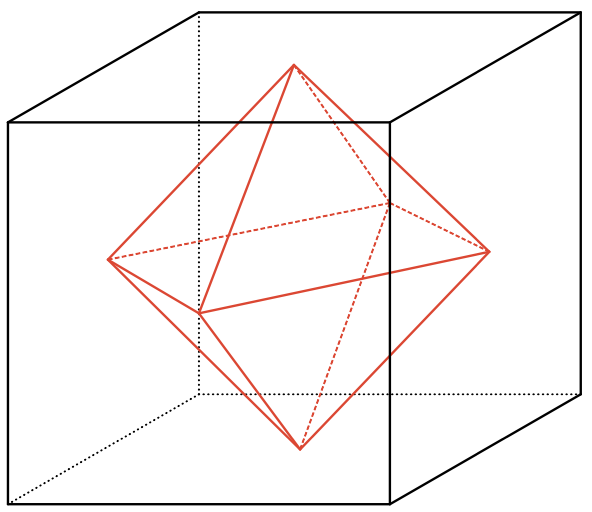
\includegraphics[width=\textwidth]{images/cube_dual.png}
%     \end{minipage}
%     \hfill
%     \begin{minipage}{0.4\textwidth}
%     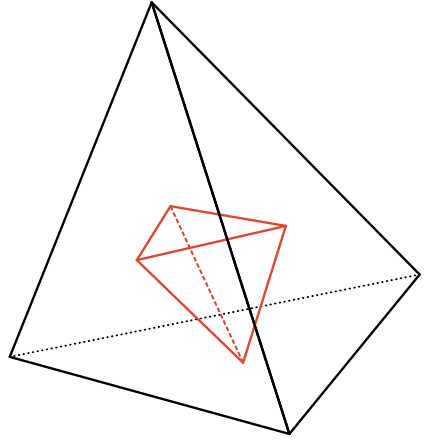
\includegraphics[width=\textwidth]{images/tetr_dual.png}
%     \end{minipage}
%     \hfill\hfill
% \end{figure}

% % asymptote starter, dots+lines
% \begin{center}
% \begin{asy}
% import graph; size(3cm); 
% pen dps = linewidth(0.7) + fontsize(10); defaultpen(dps);
% pen dotstyle = black;
% real scale = 1.75;

% pair O = (0,0);
% pair A = dir(20);
% pair pA = dir(70);

% draw(O--A);
% draw(A--pA);
% draw(O--pA);

% dot(O,dotstyle); 
% label("$O$", O, S*scale);
% dot(A,dotstyle); 
% label("$\alpha$", A, E*scale);
% dot(pA,dotstyle); 
% label("$\rho(\alpha)$", pA, NE*scale);
% \end{asy}
% \end{center}

% % asymptote starter, circles+colors+shading
% \begin{center}
% \begin{asy}
% import graph; size(2cm); 
% pen dps = linewidth(0.7) + fontsize(10); defaultpen(dps);
% pen crust = RGB(208,184,157);
% pen beef = RGB(138, 66, 14);
% pen dotstyle = 1+black;
% real scale = 1.75;
% real sc2 = 0.4;

% path A = unitcircle;
% filldraw(A, red+opacity(0.1), crust);
% path B = scale(0.1)*unitcircle;

% pair X1 = (-0.25, 0.5);
% pair X2 = (-0.25, 0);
% pair X3 = (-0.25, -0.5);
% pair X4 = (-0.67, 0.25);
% pair X5 = (-0.67, -0.25);
% filldraw(shift(X1)*B, beef, beef);
% filldraw(shift(X2)*B, beef, beef);
% filldraw(shift(X3)*B, beef, beef);
% filldraw(shift(X4)*B, beef, beef);
% filldraw(shift(X5)*B, beef, beef);
% \end{asy}
% \end{center}

% % general matrix starter
% \begin{pmatrix}3 & 2 \\ 2 & 5\end{pmatrix}
% \twotwo{1}{0}{0}{1} % id
% \vtwo{1}{0} % 2x1
% \htwo{0}{1} % 1x2

% % 3x3 matrix
% \begin{pmatrix}
% 1 & 0 & 0 \\
% 0 & 1 & 0 \\
% 0 & 0 & 1
% \end{pmatrix}

% % basis vectors vertical matrix
% \begin{pmatrix}
%     \vert & & \vert \\
%     v_1   & \hdots & v_n   \\
%     \vert & & \vert
% \end{pmatrix}

% % basis vectors horizontal matrix
% \begin{pmatrix}
%     \text{---} & v_1 & \text{---} \\
%      & \vdots & \\
%     \text{---} & v_2 & \text{---}
% \end{pmatrix}

% % 2x2 block matrix
% \[\left(\begin{array}{ c | c }
%     A & B \\
%     \hline
%     C & D
%   \end{array}\right)\]

% % more general block matrices
% % same pattern as above
% \[M = \left(
%     \begin{array}{cc}
%       \multicolumn{1}{c|}{A} & 0 \\ \cline{1-2}
%       \multicolumn{1}{c|}{0} & B \\
%     \end{array}
%     \right)\]
% % more complicated pattern 
% \[\left(
%     \begin{array}{ccccc}
%       A_{11} & 0 & \cdots & \multicolumn{1}{c|}{0} &\cdots \\
%       \cline{2-5}
%       \multicolumn{1}{c|}{0} &&&\multicolumn{1}{c|}{} &\multicolumn{1}{c|}{} \\
%       \multicolumn{1}{c|}{\vdots} && (M_{ij}) &\multicolumn{1}{c|}{} &\multicolumn{1}{c|}{} \\
%       \multicolumn{1}{c|}{0} &&&\multicolumn{1}{c|}{} &\multicolumn{1}{c|}{}\\ \cline{1-4}
%       \multicolumn{1}{c|}{\vdots} &&&& \multicolumn{1}{c|}{}\\
%       \cline{2-5}
%     \end{array}
%     \right)\]
